\documentclass[../AnalysisNoteJBuxton.tex]{subfiles}
\begin{document}

\subsection{Typical Correlation Function Construction}
\label{TypicalCfConstruction}

In practice, $B(k^{*})$ is typically obtained by forming mixed-event pairs, i.e. particles from a given event are paired with particles from N$_{mix}$(= 5) other events, and these pairs are then binned in $k^{*}$.
In forming the background distribution, it is important to mix only similar events; mixing events with different phase-spaces can result in an unreliable background distribution, and can introduce artificial signals in the correlation function.
Therefore, in this analysis, we bin our events both in primary vertex location (2 cm bin width) and in centrality (5\% bin width), and we only mix events within a given bin; i.e. we only mix events of like centrality and of like primary vertex location.
Also note, a vertex correction is also applied to each event, which essentially recenters the the primary vertices to z = 0.

Figures \ref{fig:AllCfs:a}, \ref{fig:AllCfs:b}, \ref{fig:AllCfs:c} show the correlation functions for all centralities studied for \LamKchPALamKchM, \LamKchMALamKchP, and \LamALamKs, respectively. All were normalized in the range 0.32 $< k^{*} < $ 0.4 GeV/$c$.  It is interesting to note that the average of the \LamKchPALamKchM and \LamKchMALamKchP correlation functions is consistent with our \LamKsALamKs measurement. 

\begin{figure}[h!]
  \centering
  %%----start of first subfigure---  
  \subfloat[\LamKchP (left) and \ALamKchM (right) correlations for 0-10\% (top), 10-30\%(middle), and 30-50\%(bottom) centralities.]{
    \label{fig:AllCfs:a}
    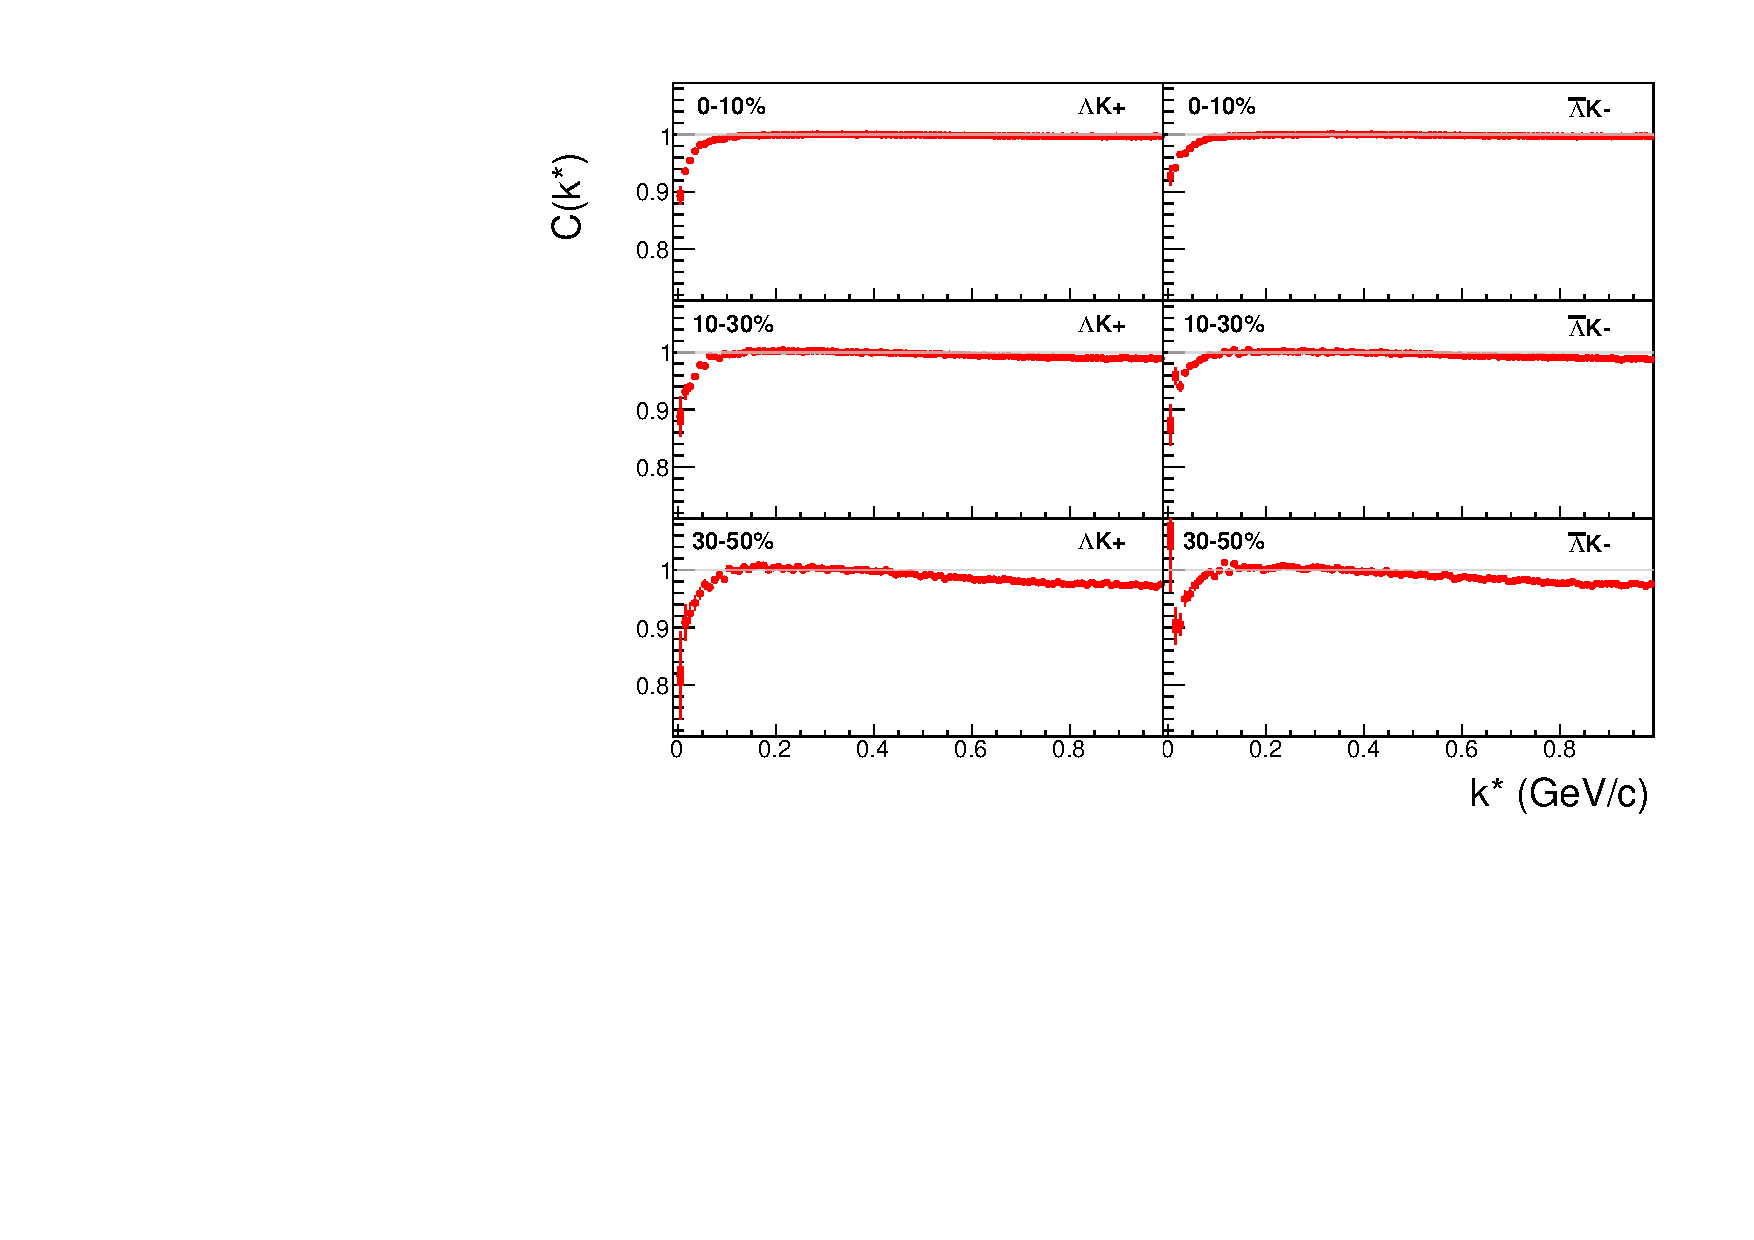
\includegraphics[width=0.49\textwidth]{4_CorrelationFunctions/Figures/canKStarCfsLamKchPwConj_0010_1030_3050.pdf}}
  %%----start of second subfigure---
  \subfloat[\LamKchM (left) and \ALamKchP (right) correlations for 0-10\% (top), 10-30\%(middle), and 30-50\%(bottom) centralities.  The peak at k* $\approx$ 0.2 GeV/c is due to the $\Omega^{-}$ (and, to a much smaller extent, the $\Xi$(1690) resonance.]{
    \label{fig:AllCfs:b}
    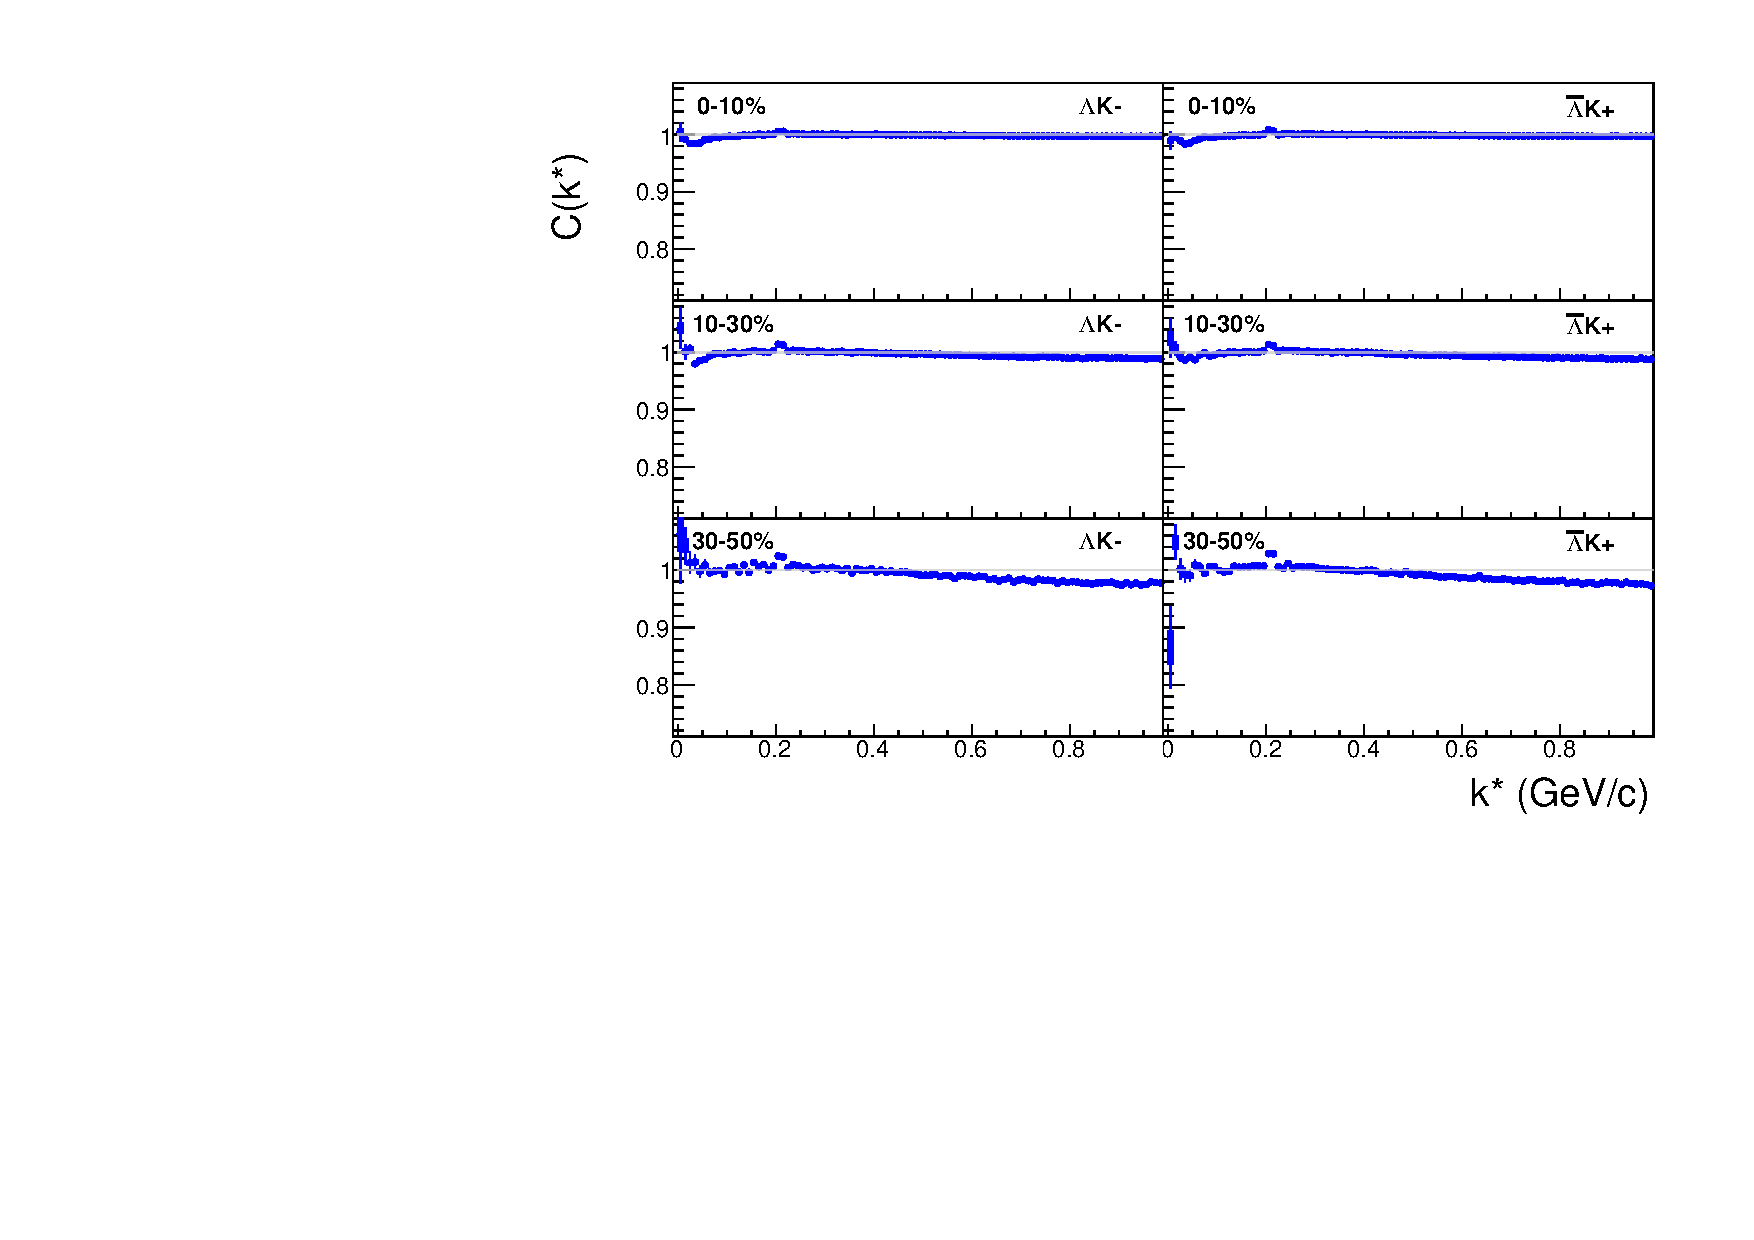
\includegraphics[width=0.49\textwidth]{4_CorrelationFunctions/Figures/canKStarCfsLamKchMwConj_0010_1030_3050.pdf}}
  \\  
  %%----start of third subfigure---
  \subfloat[\LamKs (left) and \ALamKs (right) correlations for 0-10\% (top), 10-30\%(middle), and 30-50\%(bottom) centralities.]{
    \label{fig:AllCfs:c}
    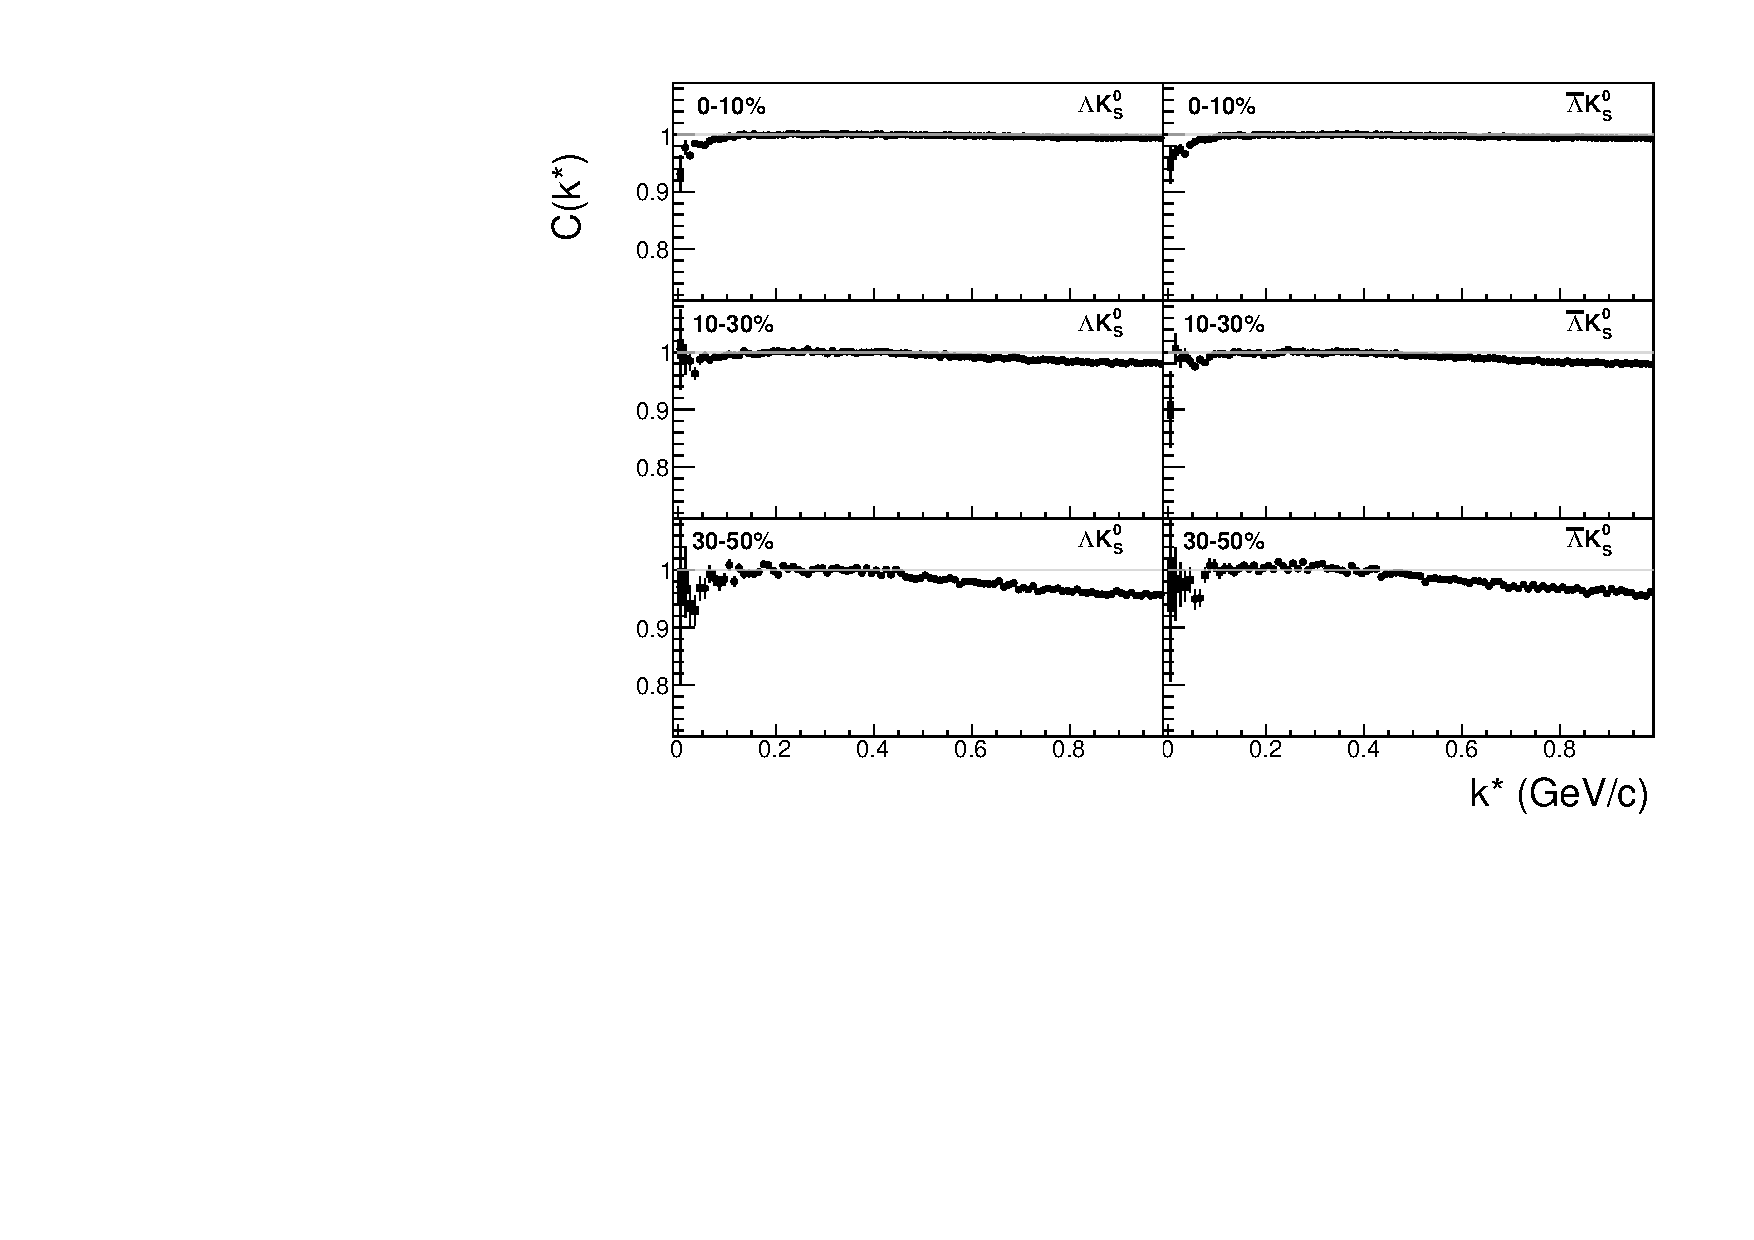
\includegraphics[width=0.49\textwidth]{4_CorrelationFunctions/Figures/canKStarCfsLamK0wConj_0010_1030_3050.pdf}}    
  %%----overall caption----
  \caption[\LamK Correlation Functions]{\LamK and \ALamAK correlation functions for 0-10\%, 10-30\%, and 30-50\% centralities.  The lines represent the statistical errors, while the boxes represent the systematic errors.}
  \label{fig:AllCfs}
\end{figure}


\begin{figure}[h]
  \centering
  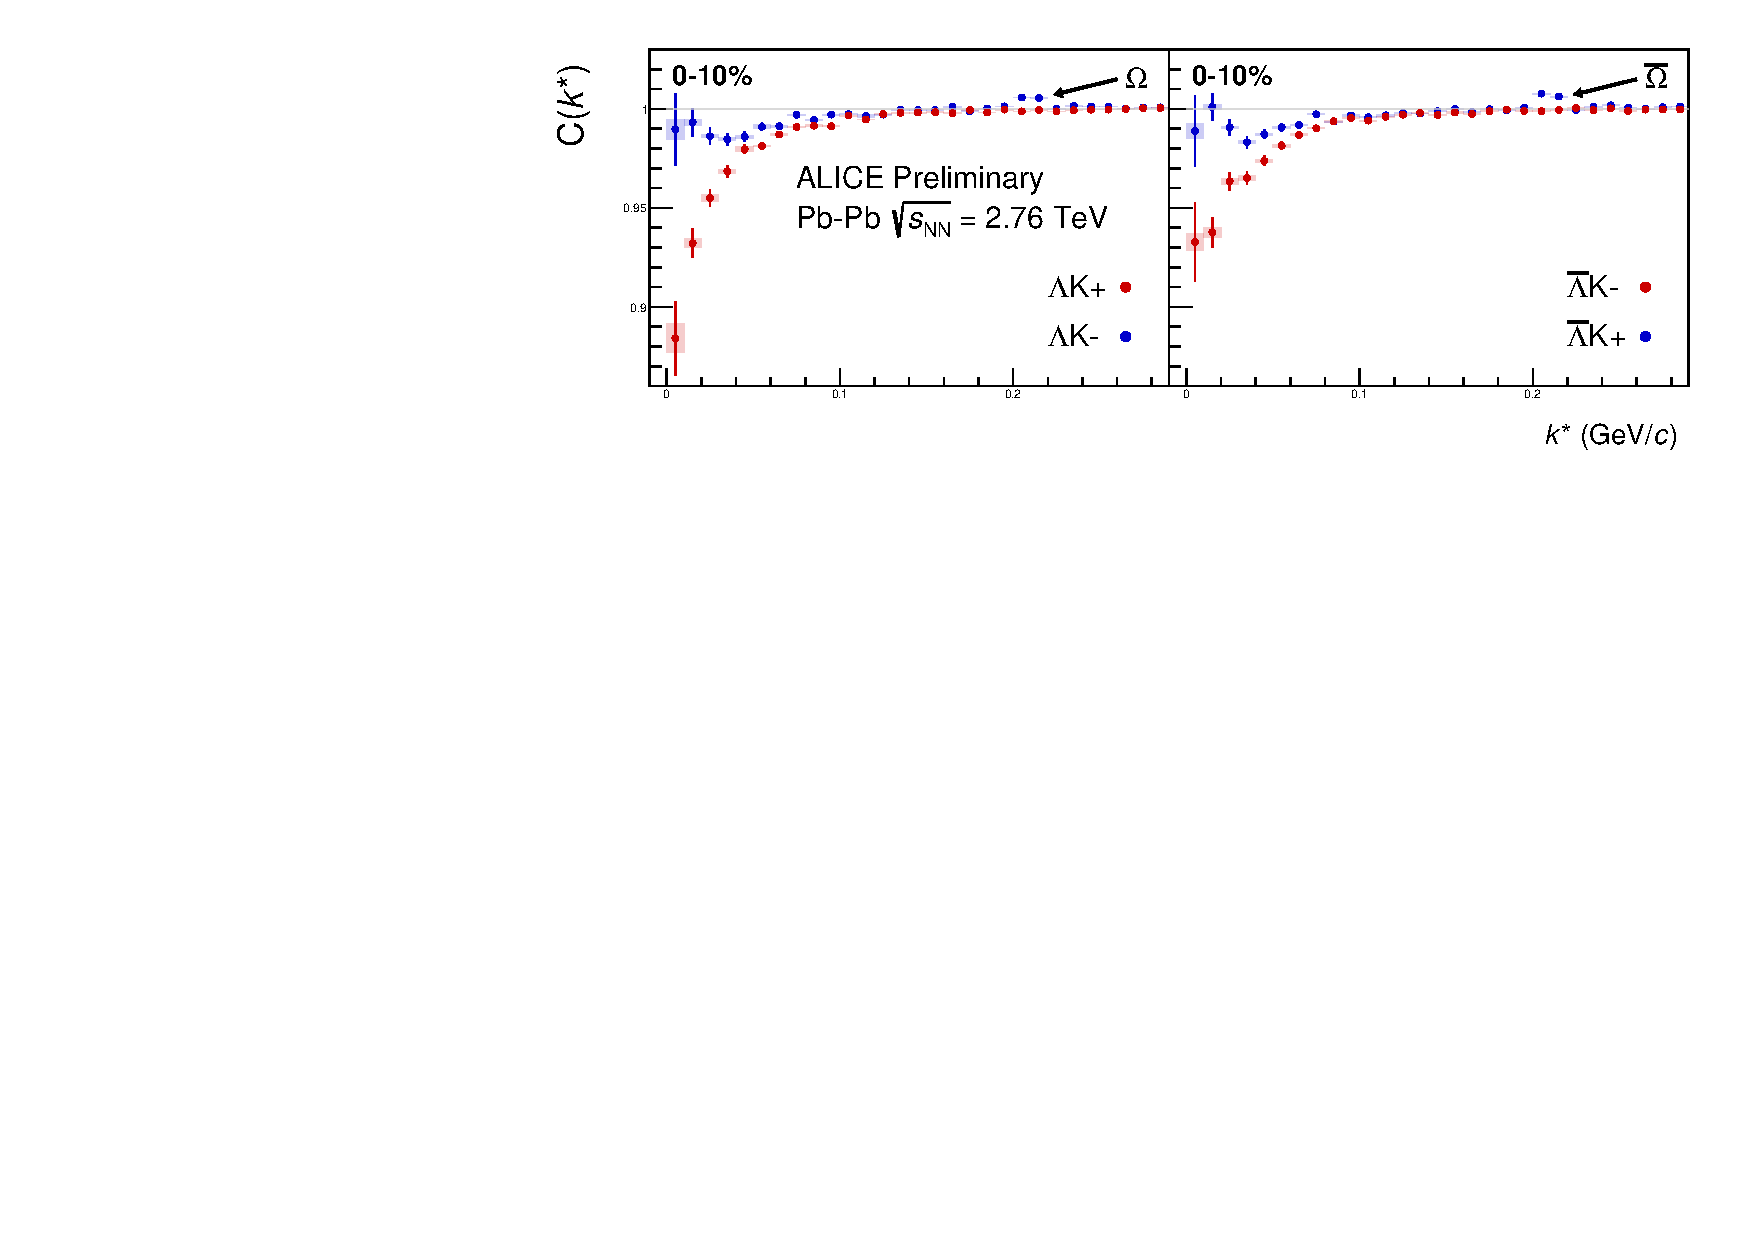
\includegraphics[width=\textwidth]{4_CorrelationFunctions/Figures/canLamKchPvsLamKchM0010.pdf}
  \caption[Correlation Functions: \LamKchP vs \LamKchM for 0-10\% Centrality]{Correlation Functions: \LamKchP vs \LamKchM (\ALamKchP vs \ALamKchM) for 0-10\% centrality.  The peak in \LamKchMALamKchP at \kstar $\approx$ 0.2 GeV/c is due to the $\Omega^{-}$ (and, to a much smaller extent, the $\Xi$(1690) resonance.  The lines represent the statistical errors, while boxes represent systematic errors.}
  \label{fig:cLamcKchCfs0010}
\end{figure}

\clearpage

\end{document}